\section{Ciclo de vida de software}
\label{sec:ciclo}


Engenheiros de software tem tradicionalmente considerado qualquer trabalho após
o primeiro lançamento de um software simplesmente como manutenção. Alguns
pesquisadores no entanto tem dividido este trabalho em atividades distintas, incluindo
adaptação, prevenção, correção, entre outras, mas sempre considerando manutenção
basicamente uniforme ao longo do tempo \cite{rajlich2000staged}.

Entretanto, alguns estudos tem demonstrado que esta visão, onde manutenção
ocupa um papel basicamente uniforme ao longo do tempo, não explica muito bem o
desenvolvimento de software na maior parte dos cenários, e uma das abordagens
para explicar o fenômeno tem colocado a atividade de manutenção distribuída ao
longo do ciclo de vida do software \cite{rajlich2000staged}.

Este modelo de evolução do software em estágios, no entanto, foi avaliado e adaptado
ao contexto de software livre \cite{capiluppi2007adapting}, e diante as
semelhanças com o software acadêmico, este modelo adaptado ao software livre serve ao propósito de ser
utilizado para
avaliar a evolução do software acadêmico, a Figura \ref{staged-model-foss-cycle}
apresenta o modelo de evolução adaptado ao software livre, adotado
neste estudo como aplicável também ao software acadêmico.

\begin{figure}[h]
  \center
  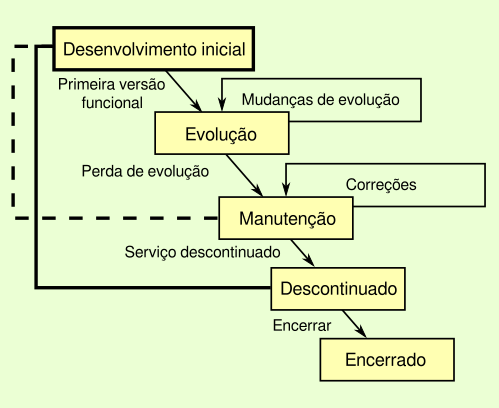
\includegraphics[scale=0.6]{imagens/staged-model-foss-cycle.png}
  \caption{O modelo de evolução {\it staged model} adaptado a software livre \cite{capiluppi2007adapting}.}
  \label{staged-model-foss-cycle}
\end{figure}

A primeira diferença observada é em relação a fase {\it Initial development},
dependendo da definição de ``fase inicial'' muitos projetos de software livre
podem nunca ter saído desta fase, assim é também para o software acadêmico. Em respeito aos lançamentos,
em sistemas comerciais tradicionais eles devem ser completos, rodando e autorizado
pela empresa detentora, enquanto no mundo do software livre é comum
permitir acesso público ao código em repositórios de código fonte, seguindo
um modelo de ``versão permanente''.

A segunda diferença é relacionada a possibilidade de laços entre
as fases {\it Evolution} e {\it Servicing}. Muitos projetos de software livre
possuem fases de congelamento na adição de novas funcionalidades ({\it freeze})
enquanto permanece numa fase de {\it Servicing} até o descongelamento, voltando
a {\it Evolution}.

A terceira diferença está na comunidade de software livre,
novos times de desenvolvimento são formados ao longo do tempo
com a saída de desenvolvedores antigos e a entrada de novos.
E projetos em fase {\it Phaseout} podem experimentar um renascimento
retornando ao período de {\it Evolution}.

Apesar das diferenças, o autor \citeonline{capiluppi2007adapting} demonstram em experimentos e
revisão de literatura que o modelo adaptado pode ser utilizado para
compreender evolução de software livre, e diante as similaridades entre software livre
e software acadêmico, este modelo poderá, consequentemente, ser também
utilizado para compreender a evolução e ciclo de vida do software acadêmico.
